\htwo{Handbuch Client}
\hthree{Verwendung}
Nachdem ein ZELIA Server gestartet wurde, kann man auf das ZELIA Frontend mit einem Webbrowser zugreifen. Dafür muss man nur die IP-Adresse oder den Domainnamen eines Servers kennen, \zb\ \emph{https://szu.zelia.at/}, \emph{https://[IP-Adresse]/} oder wenn es ein Server im Entwicklungsmodus ist \emph{https://localhost:3000/}.

Auf Smartphones hat die ZELIA Startseite einen Knopf um eine Raumnummer einzusacnnen (siehe Abbildung \ref{fig:zeliastart}). Wenn die Webseite von einem Computer aufgerufen wird, gibt es diesen Knopf nicht. Sonst sind die gesammten Webseiten aber am Computer und Smartphone gleich aufgebaut.

\begin{figure}[H]
    \centering
    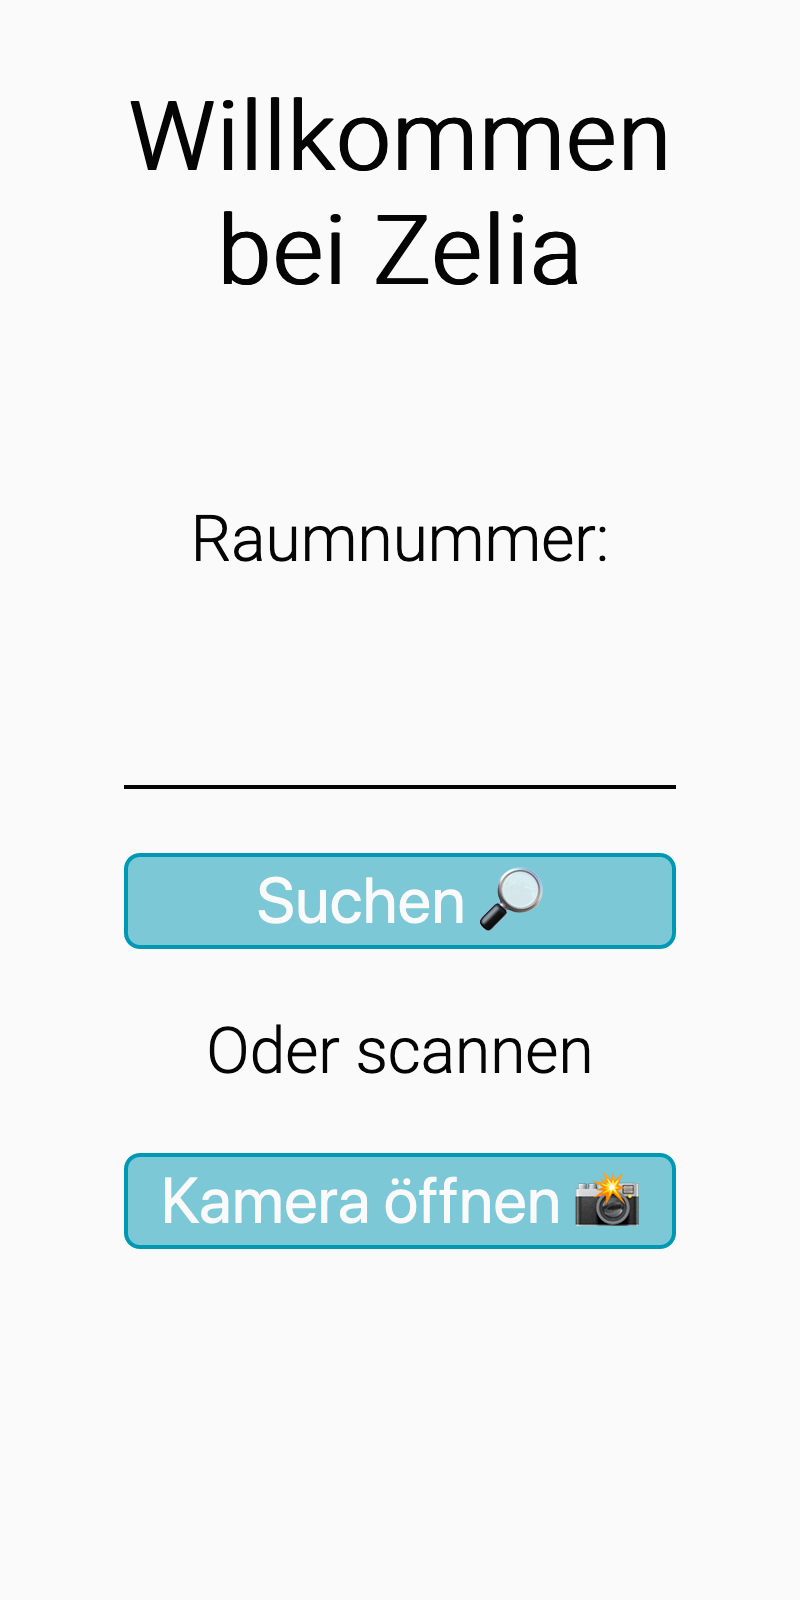
\includegraphics[height=90mm]{media/Handbuch/zelia_start.png}
    \caption{ZELIA Startseite auf Mobilgeräten}
    \label{fig:zeliastart}
\end{figure}

Auf dieser Startseite hat man die Möglichkeit eine Raumnummer einzugeben oder einzuscannen um auf die Rauminformationsseite zu gelangen. Wie im Kapitel "Die Startseite" \ref{sec:webcompstart} beschrieben, bekommt man anhand der manuellen Eingabe vorschlägen welche Räume es gibt (siehe Abbildung \ref{fig:compinput}). 

Die Rauminformationsseite zeigt zum einem Daten über einen Raum an, wie Anzahl an Plätzen oder Computern, und zum Anderen den aktuellen Stundenplan. Mit dem "Home"-Link kann man zurück auf die Startseite zurückkehren. Die Emojis zeigen auf einem Blick was in diesem Raum möglich ist. Zum Beispiel ob der Raum für Rollstuhlfahrer*innen geeignet ist oder ob ein Waschbecken vorhanden ist. Wenn man auf diese Emojis drückt, klappt man eine Auflistung auf, in der eine genauere Beschreibung des Raumes steht.

\begin{figure}[H]
    \centering
    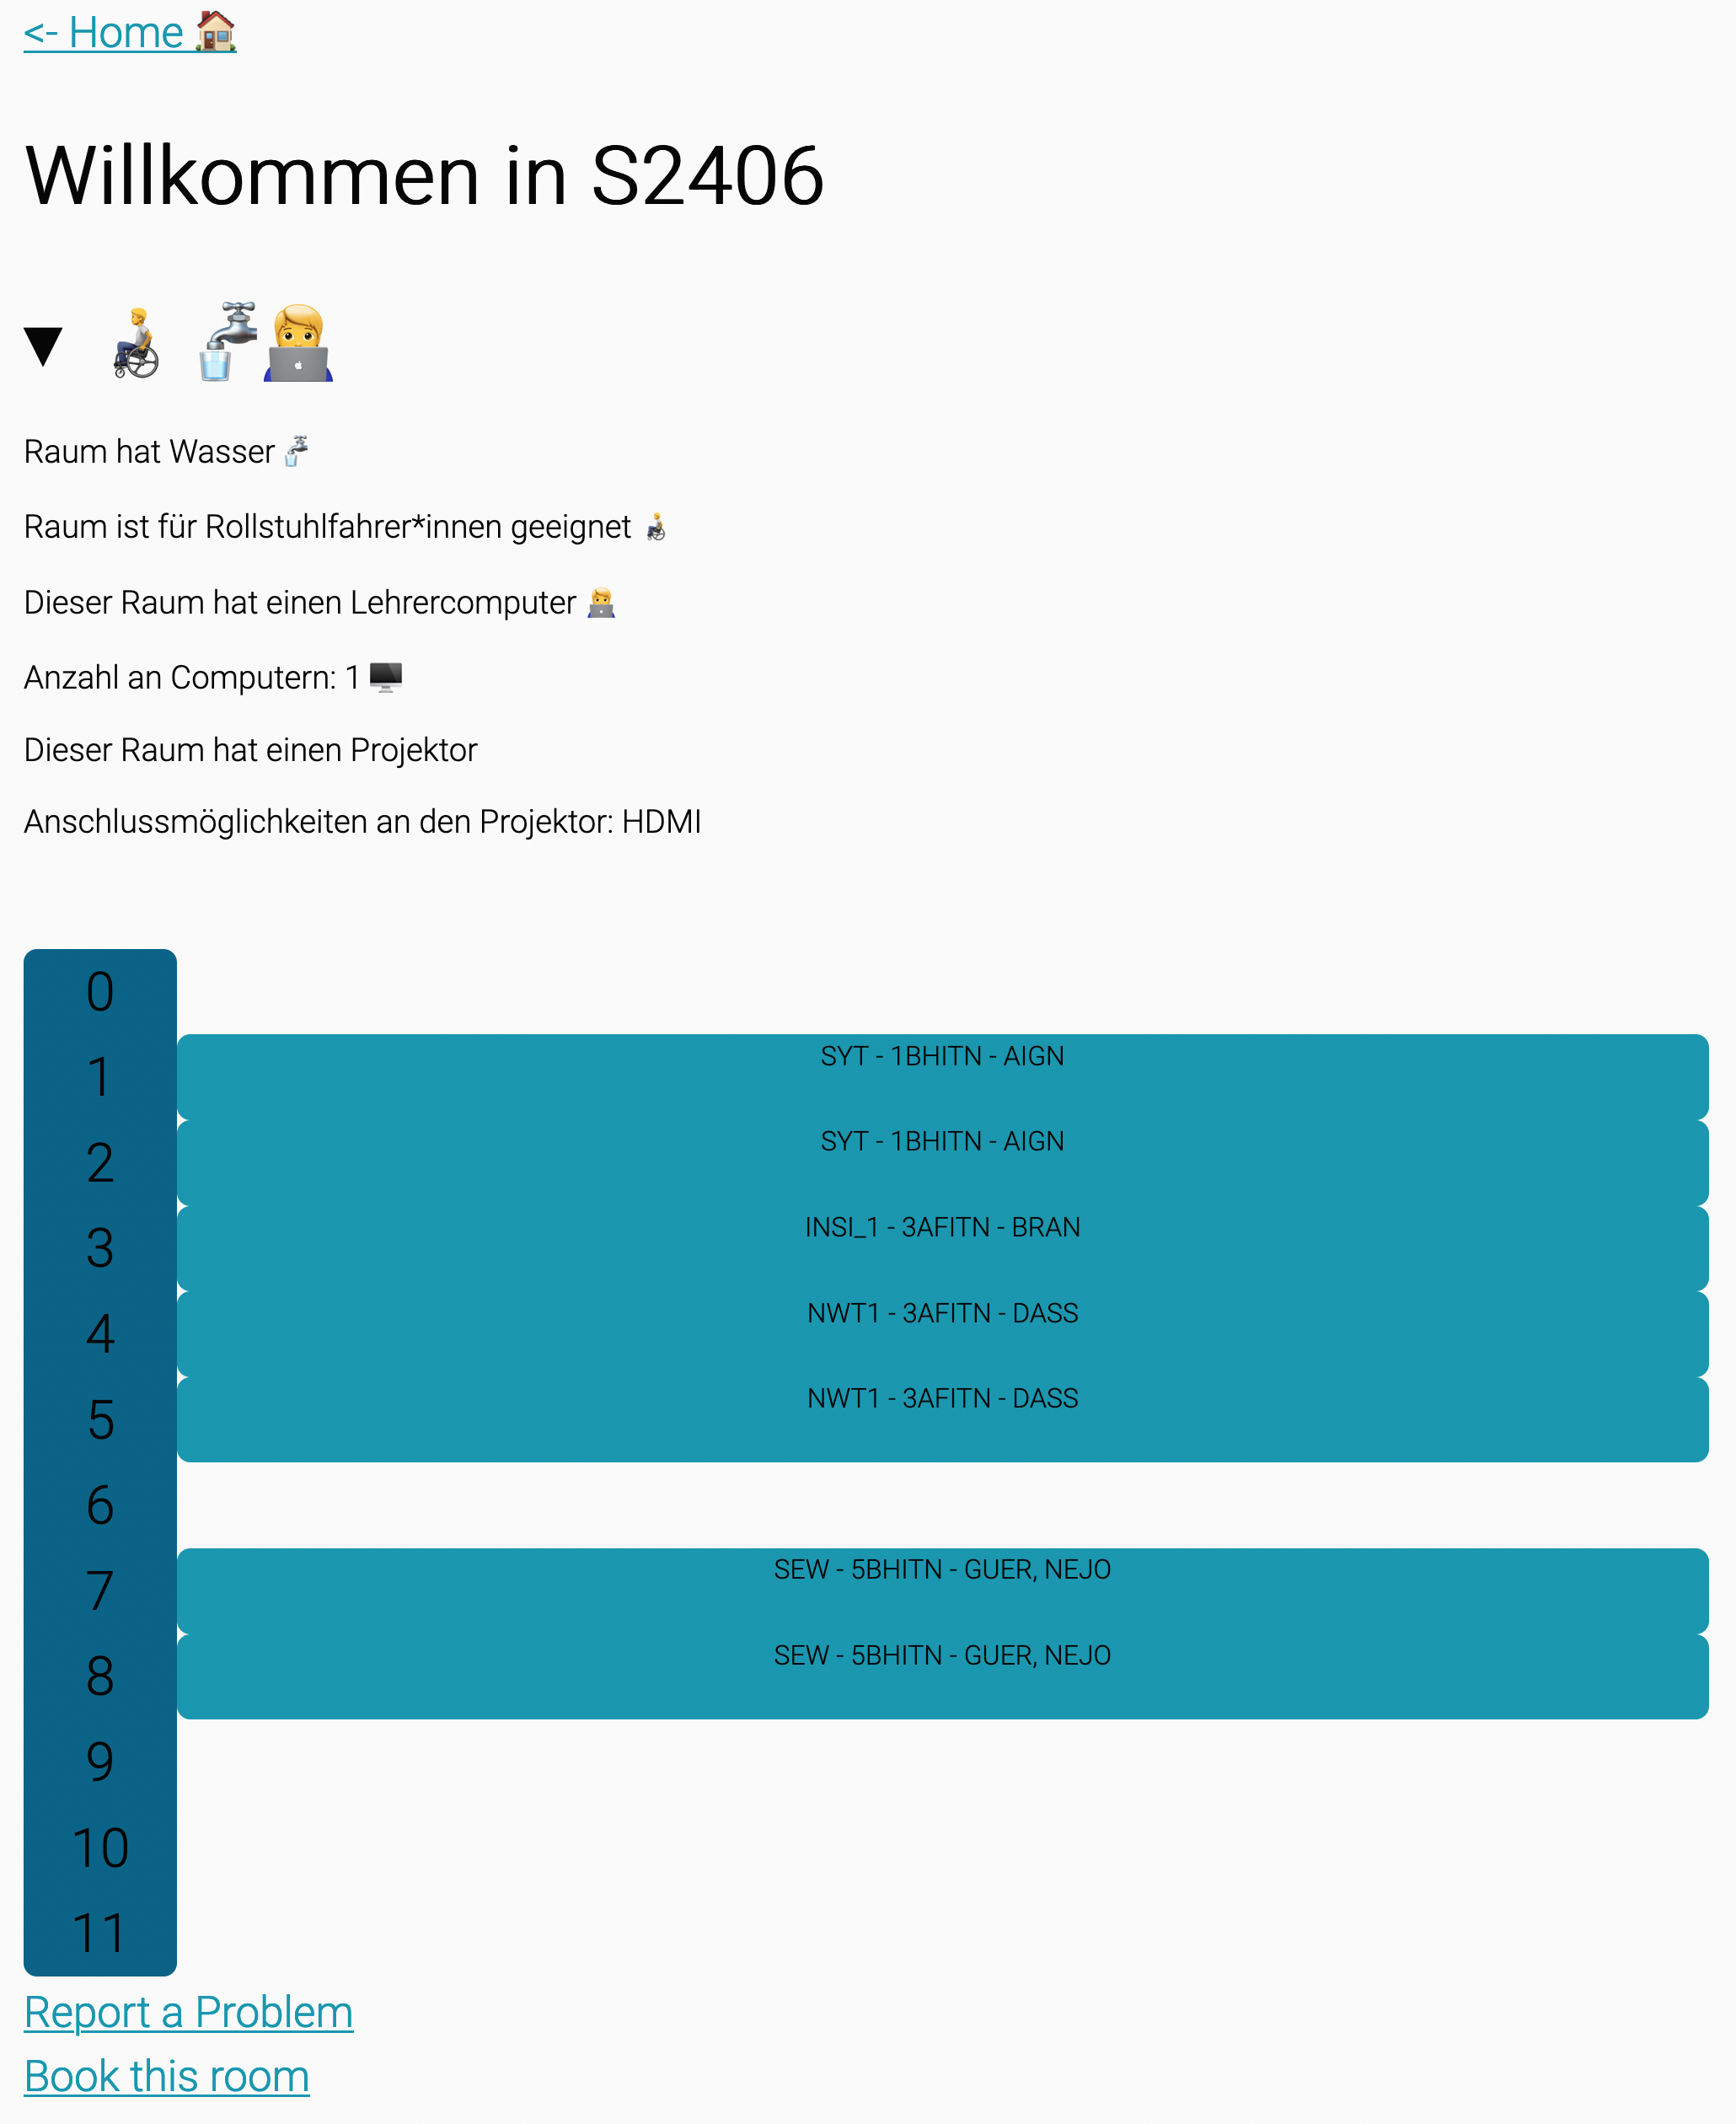
\includegraphics[width=120mm]{media/WebComponents/Rauminformationsseite_light.png}
    \caption{ZELIA Infomationsseite auf Computern}
    \label{fig:zeliainfopage}
\end{figure}

Ganz unten auf der Seite sind 2 "Links" mit den Namen "Raum melden" und "Raum buchen", welche auf die jeweilige Raumbuchungs- oder Raummeldungsseite umleiten. Diese beiden Seiten sind ähnlich aufgebaut. Sie bestehen aus einem Formular, um die Daten anzugeben die notwendig sind. Um den Meldungs- oder Buchungsvorgang abzubrechen gibt es links oben einen Link um auf die Übersichtsseite zurückzukehren.

\begin{figure}[H]
    \centering
    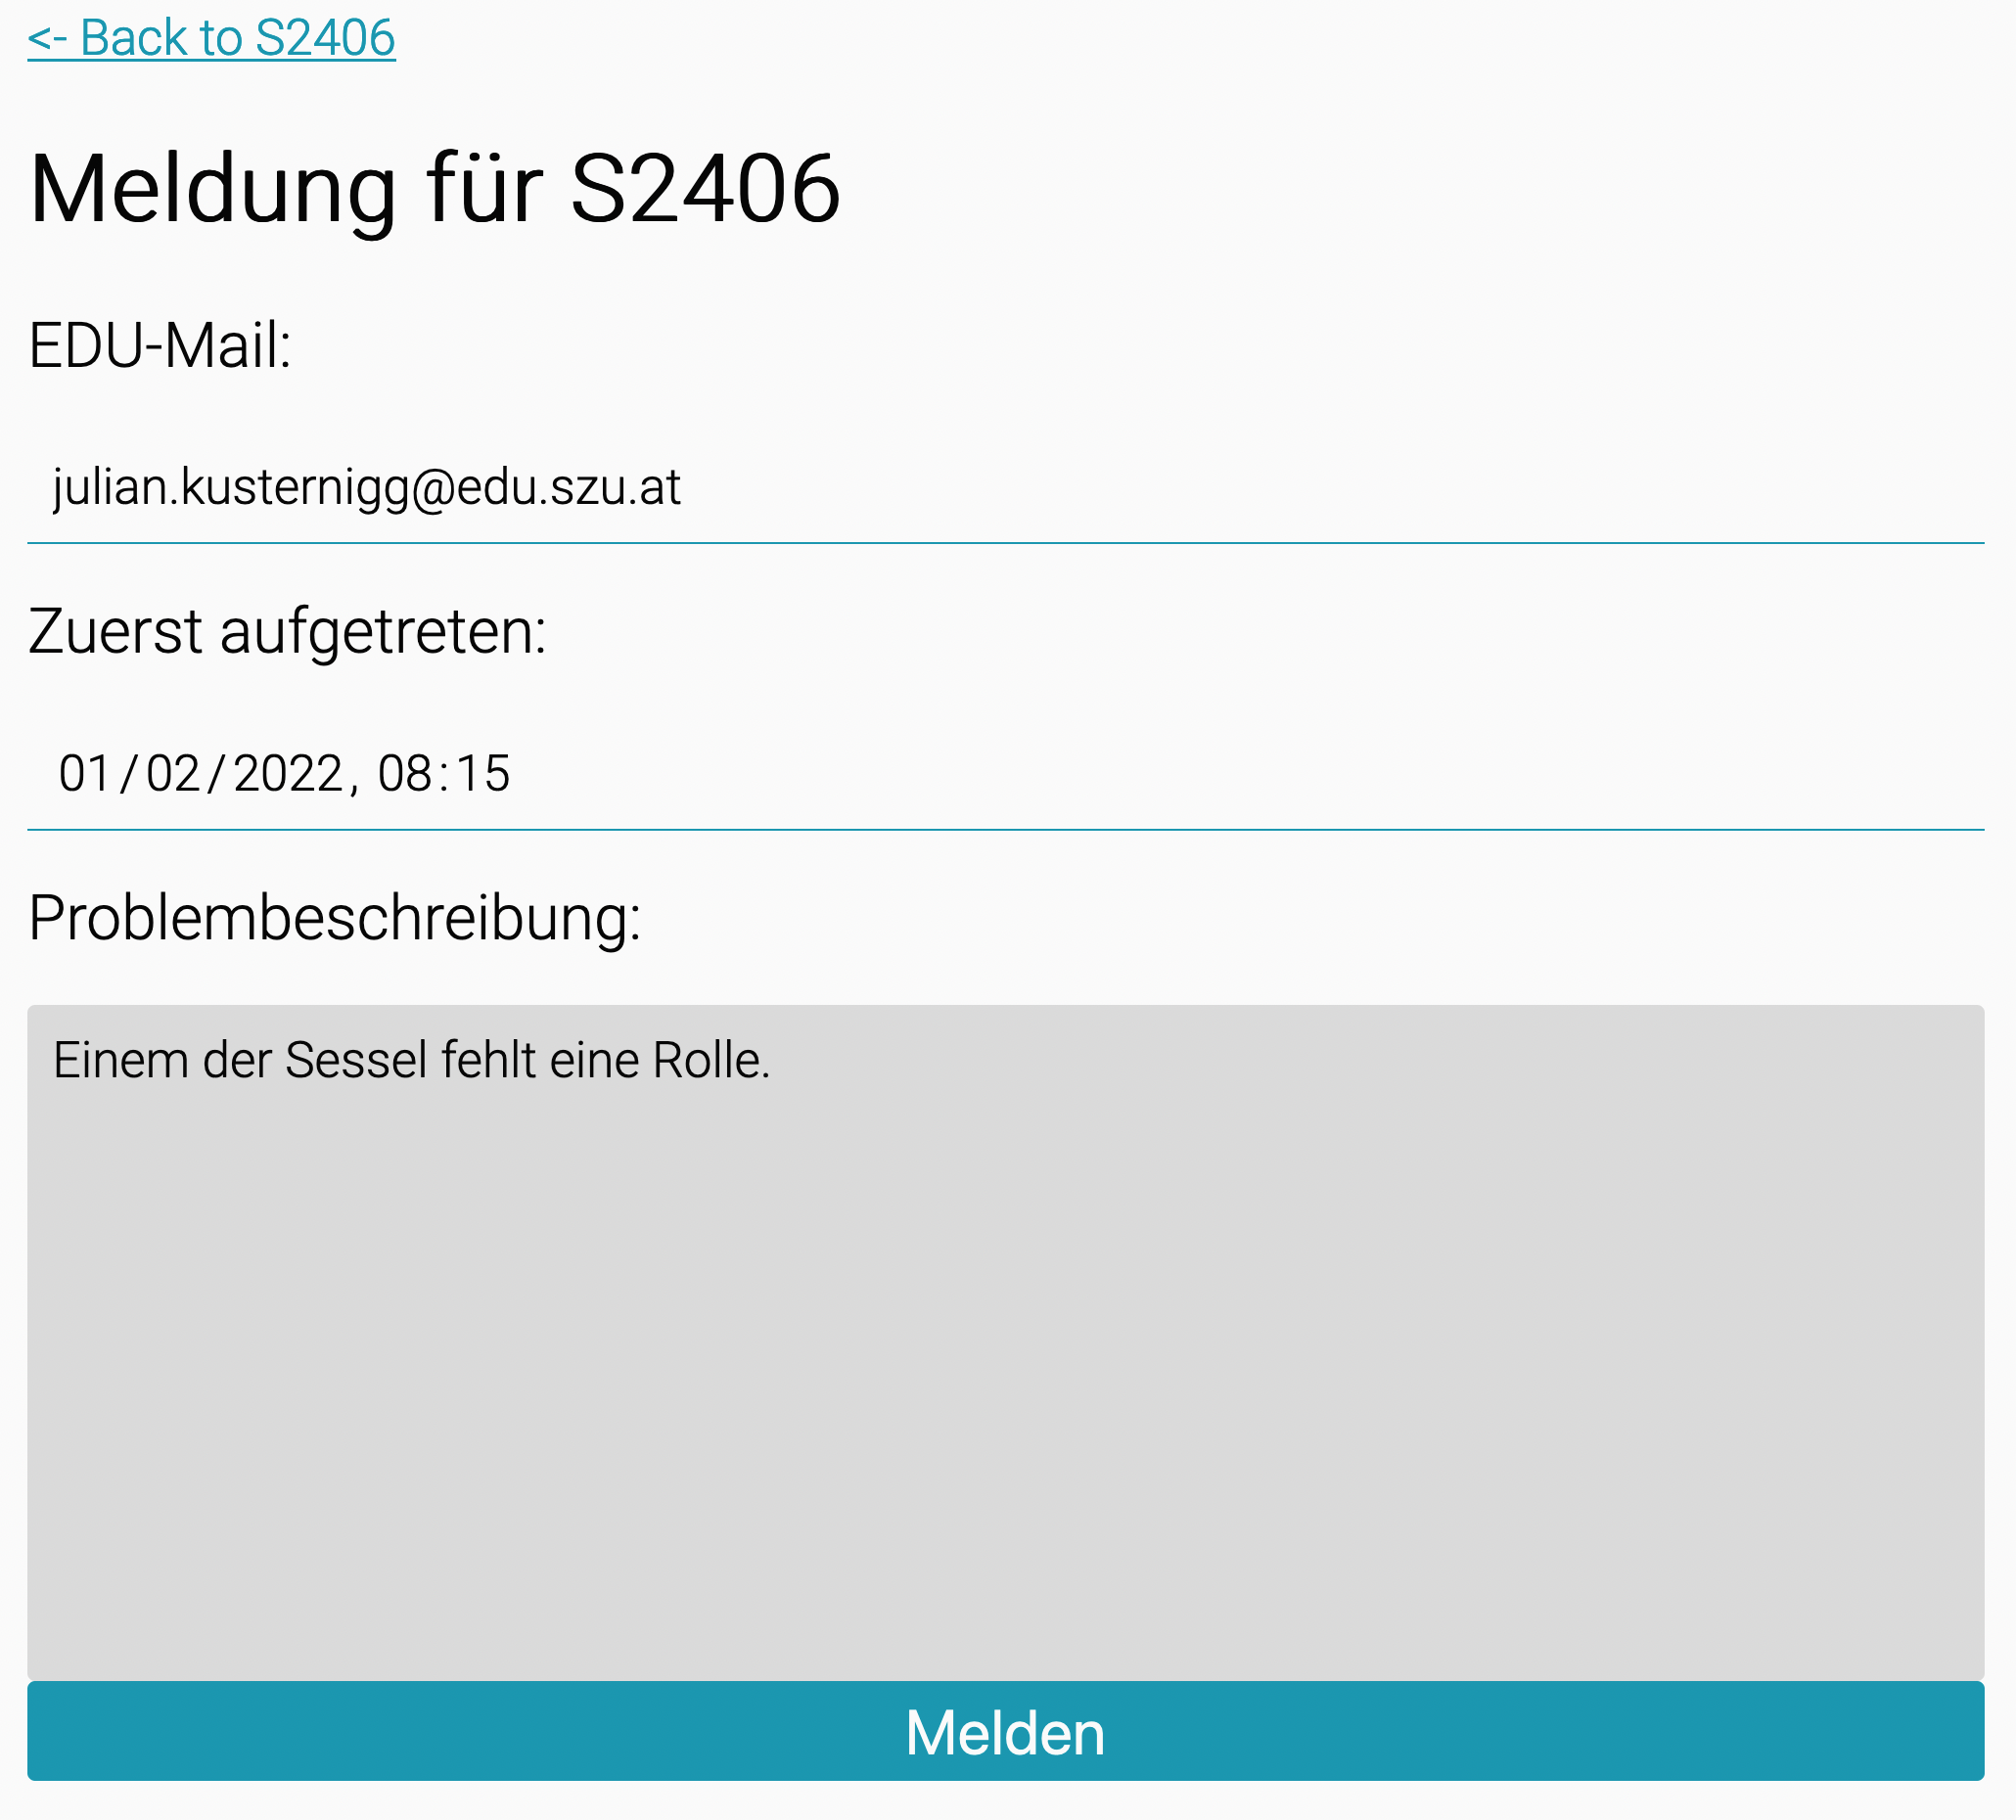
\includegraphics[width=80mm]{media/WebComponents/Meldungsseite_light.png}
    \caption{ZELIA Meldungsseite}
    
\end{figure}

\begin{figure}[H]
    \centering
    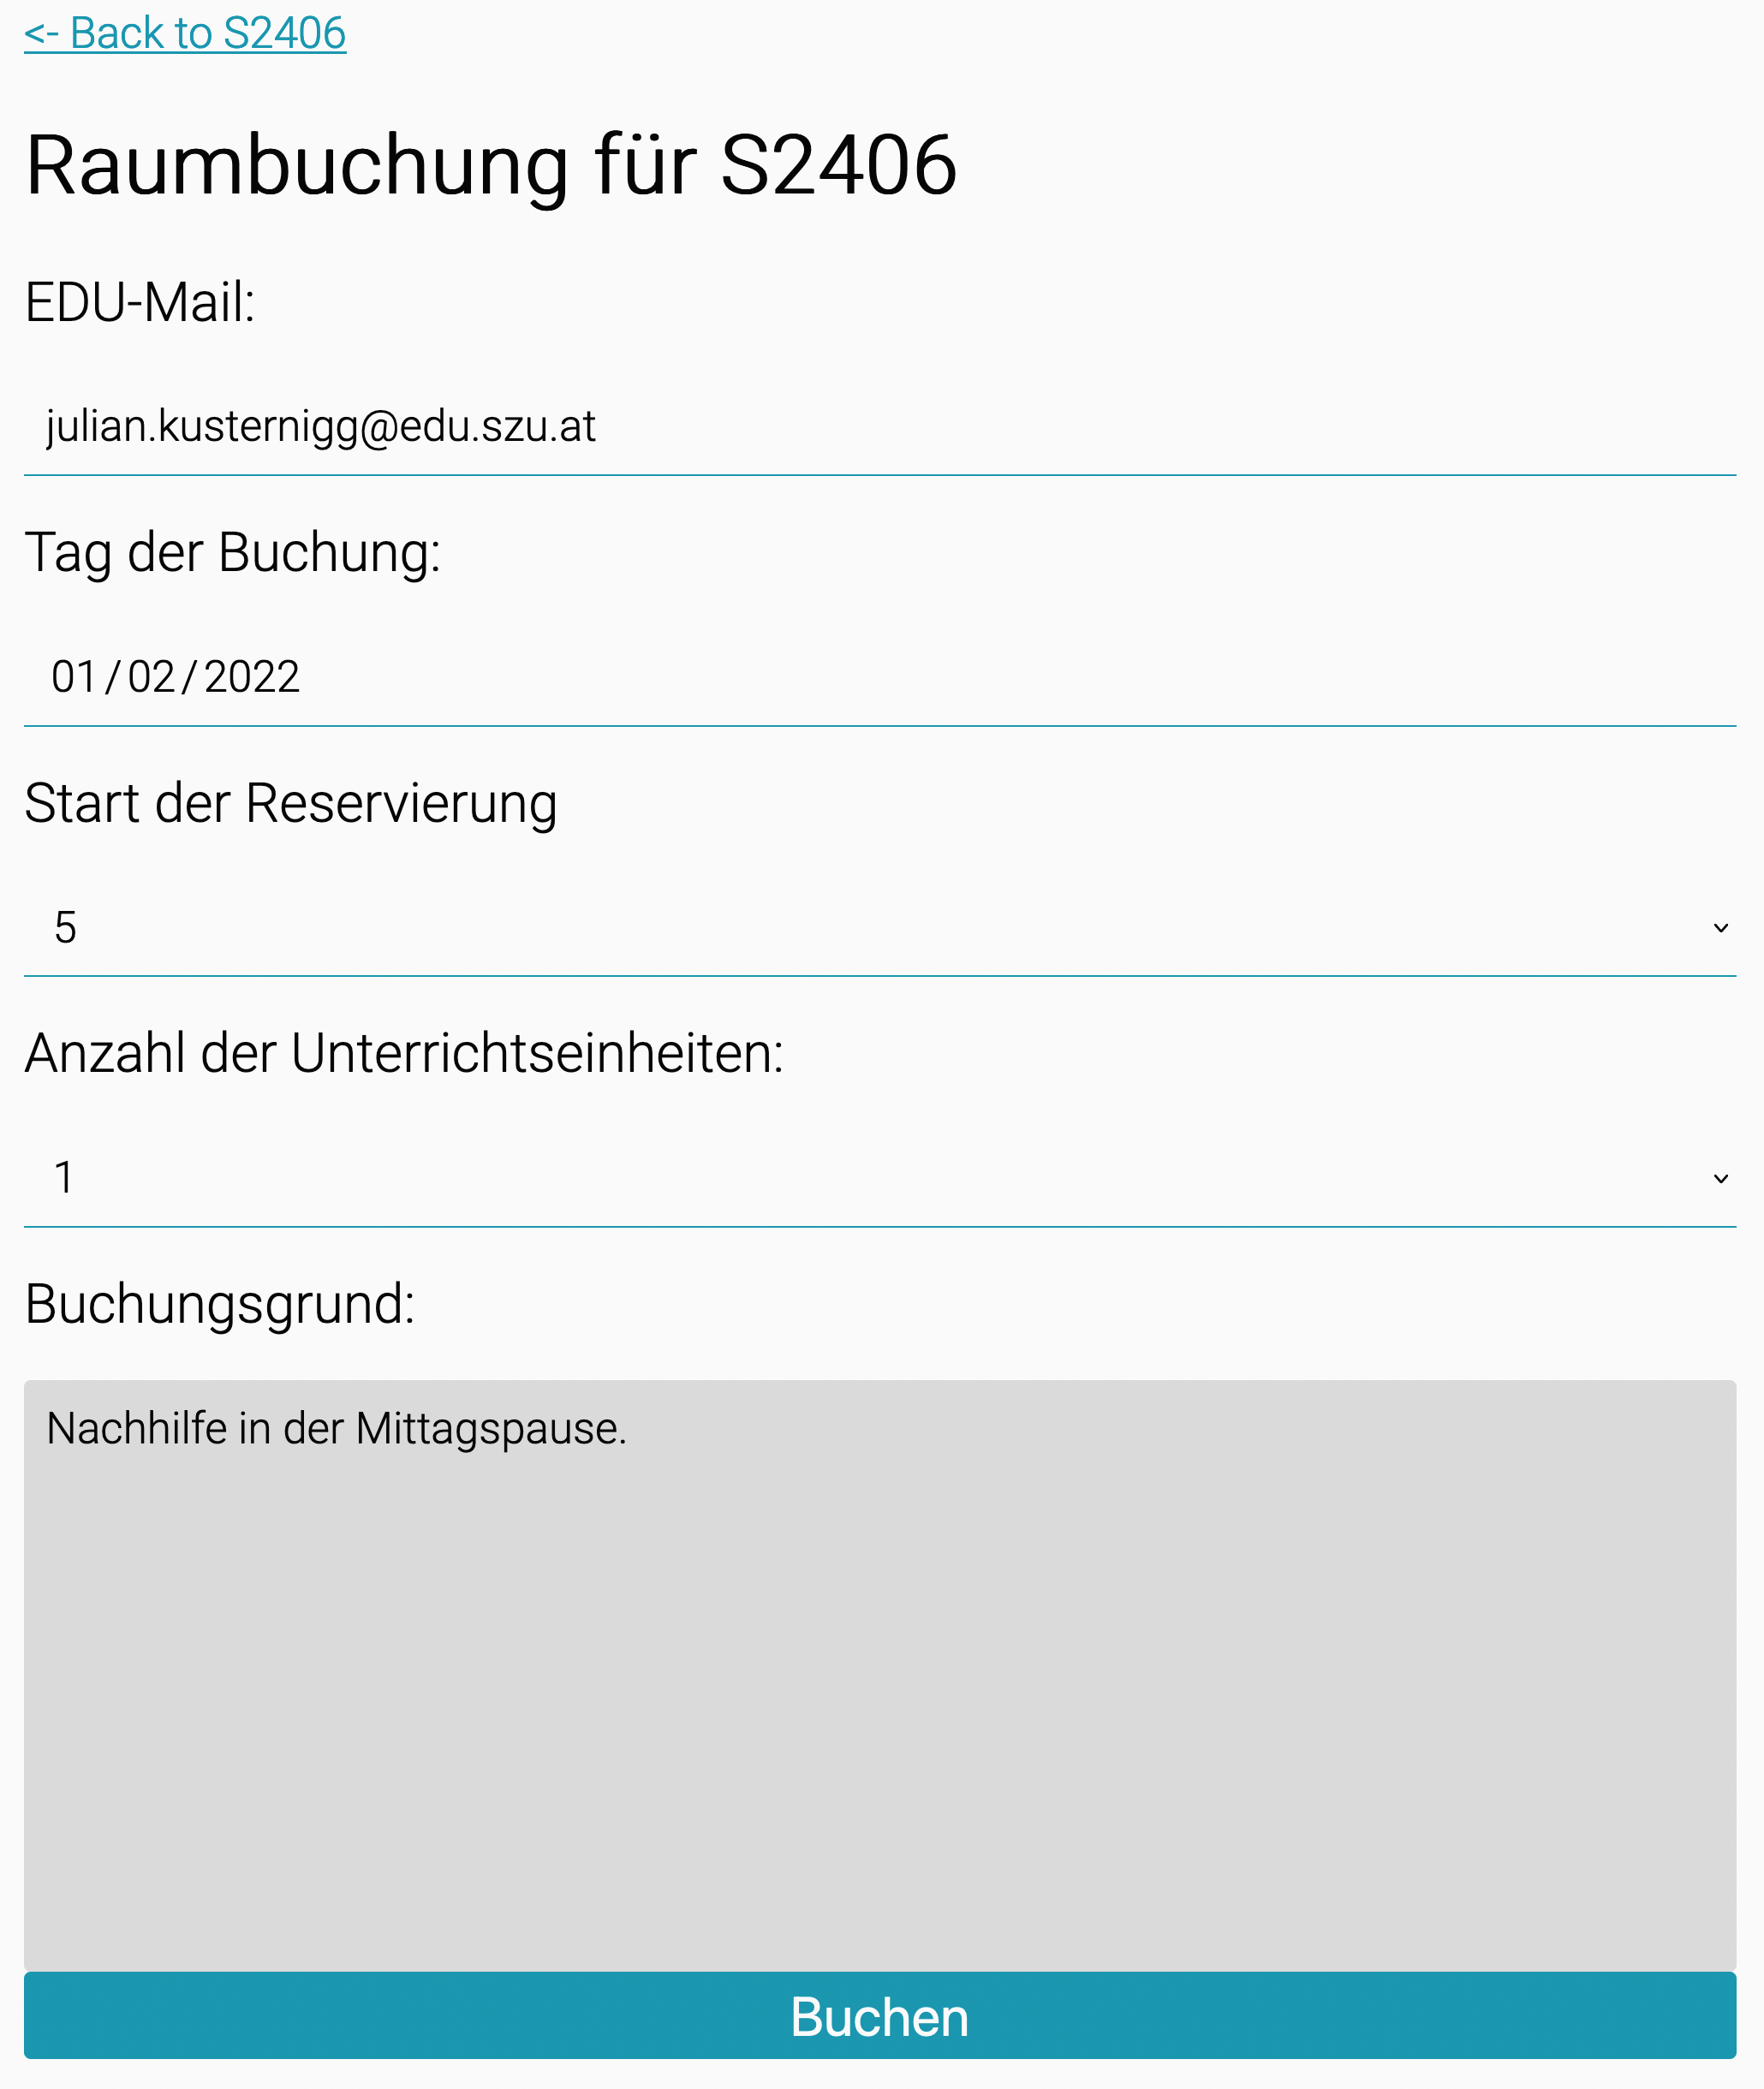
\includegraphics[width=80mm]{media/WebComponents/Buchungsseite_light.png}
    \caption{ZELIA Buchungsseite}
\end{figure}

Nachdem man das Formular abgeschickt hat und die Meldung oder Buchung mit dem Link aus der Bestätigungsemail verifiziert hat, können Lehrer*innen die angegebenen Daten in der Adminübersicht sehen.

\hthree{Admin Verwendung}

Lehrer*innen können mit Administartorbenutzern die Meldungen und Buchungen ihrer zugeordneden Klassen ansehen und abarbeiten. Dafür müssen sie den Pfad \emph{/admin} manuell in die Suchleiste eingeben. Auf dieser Seite befindet sich ein Anmeldeformular, in das der jeweilige Administartor, gültige Zugangsdaten eingaben muss, welche vom ZELIA-Administartor vergeben werden. 

\begin{figure}[H]
    \centering
    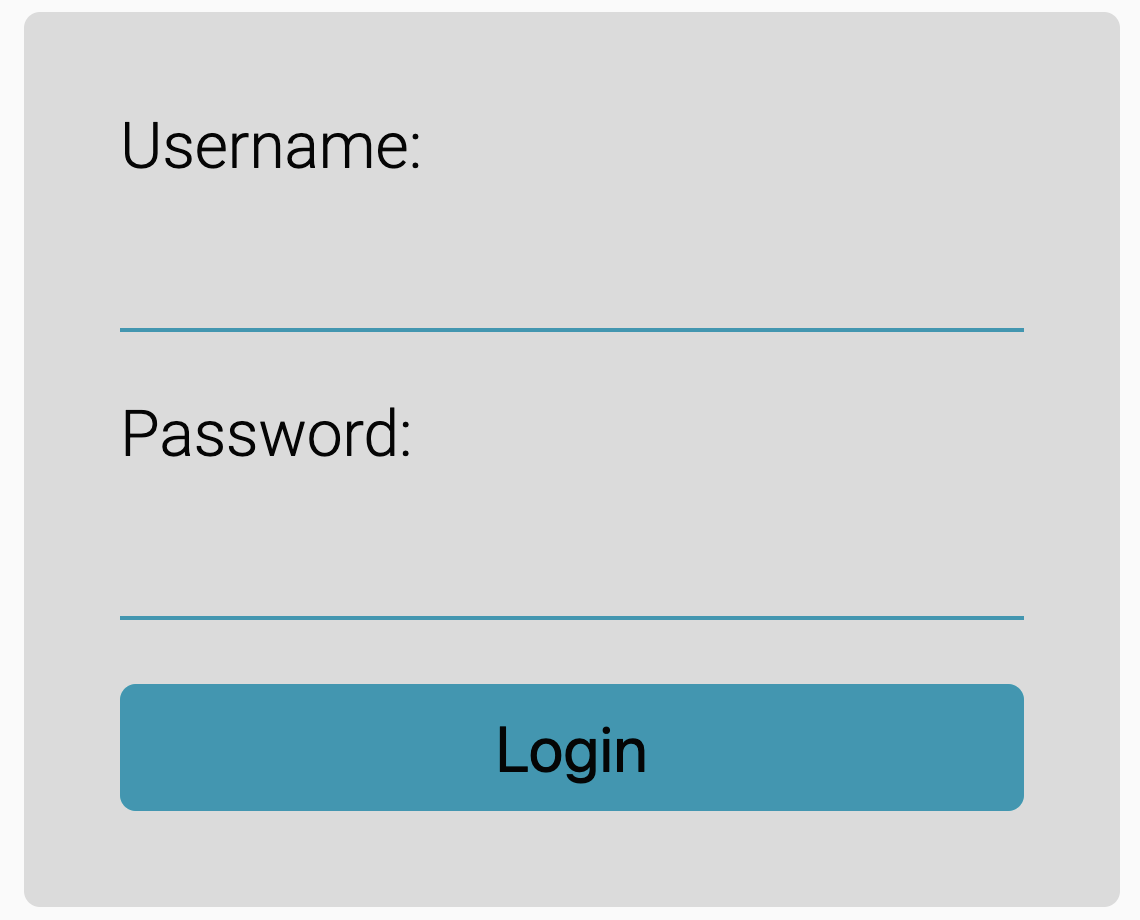
\includegraphics[width=80mm]{media/WebComponents/Login_light.png}
    \caption{ZELIA Admin Anmeldeformular}
\end{figure}

Nachdem die Anmeldung erfolgreich war, sieht man die Adminübersicht, auch genannt "Admin Dashboard". 

\begin{figure}[H]
    \centering
    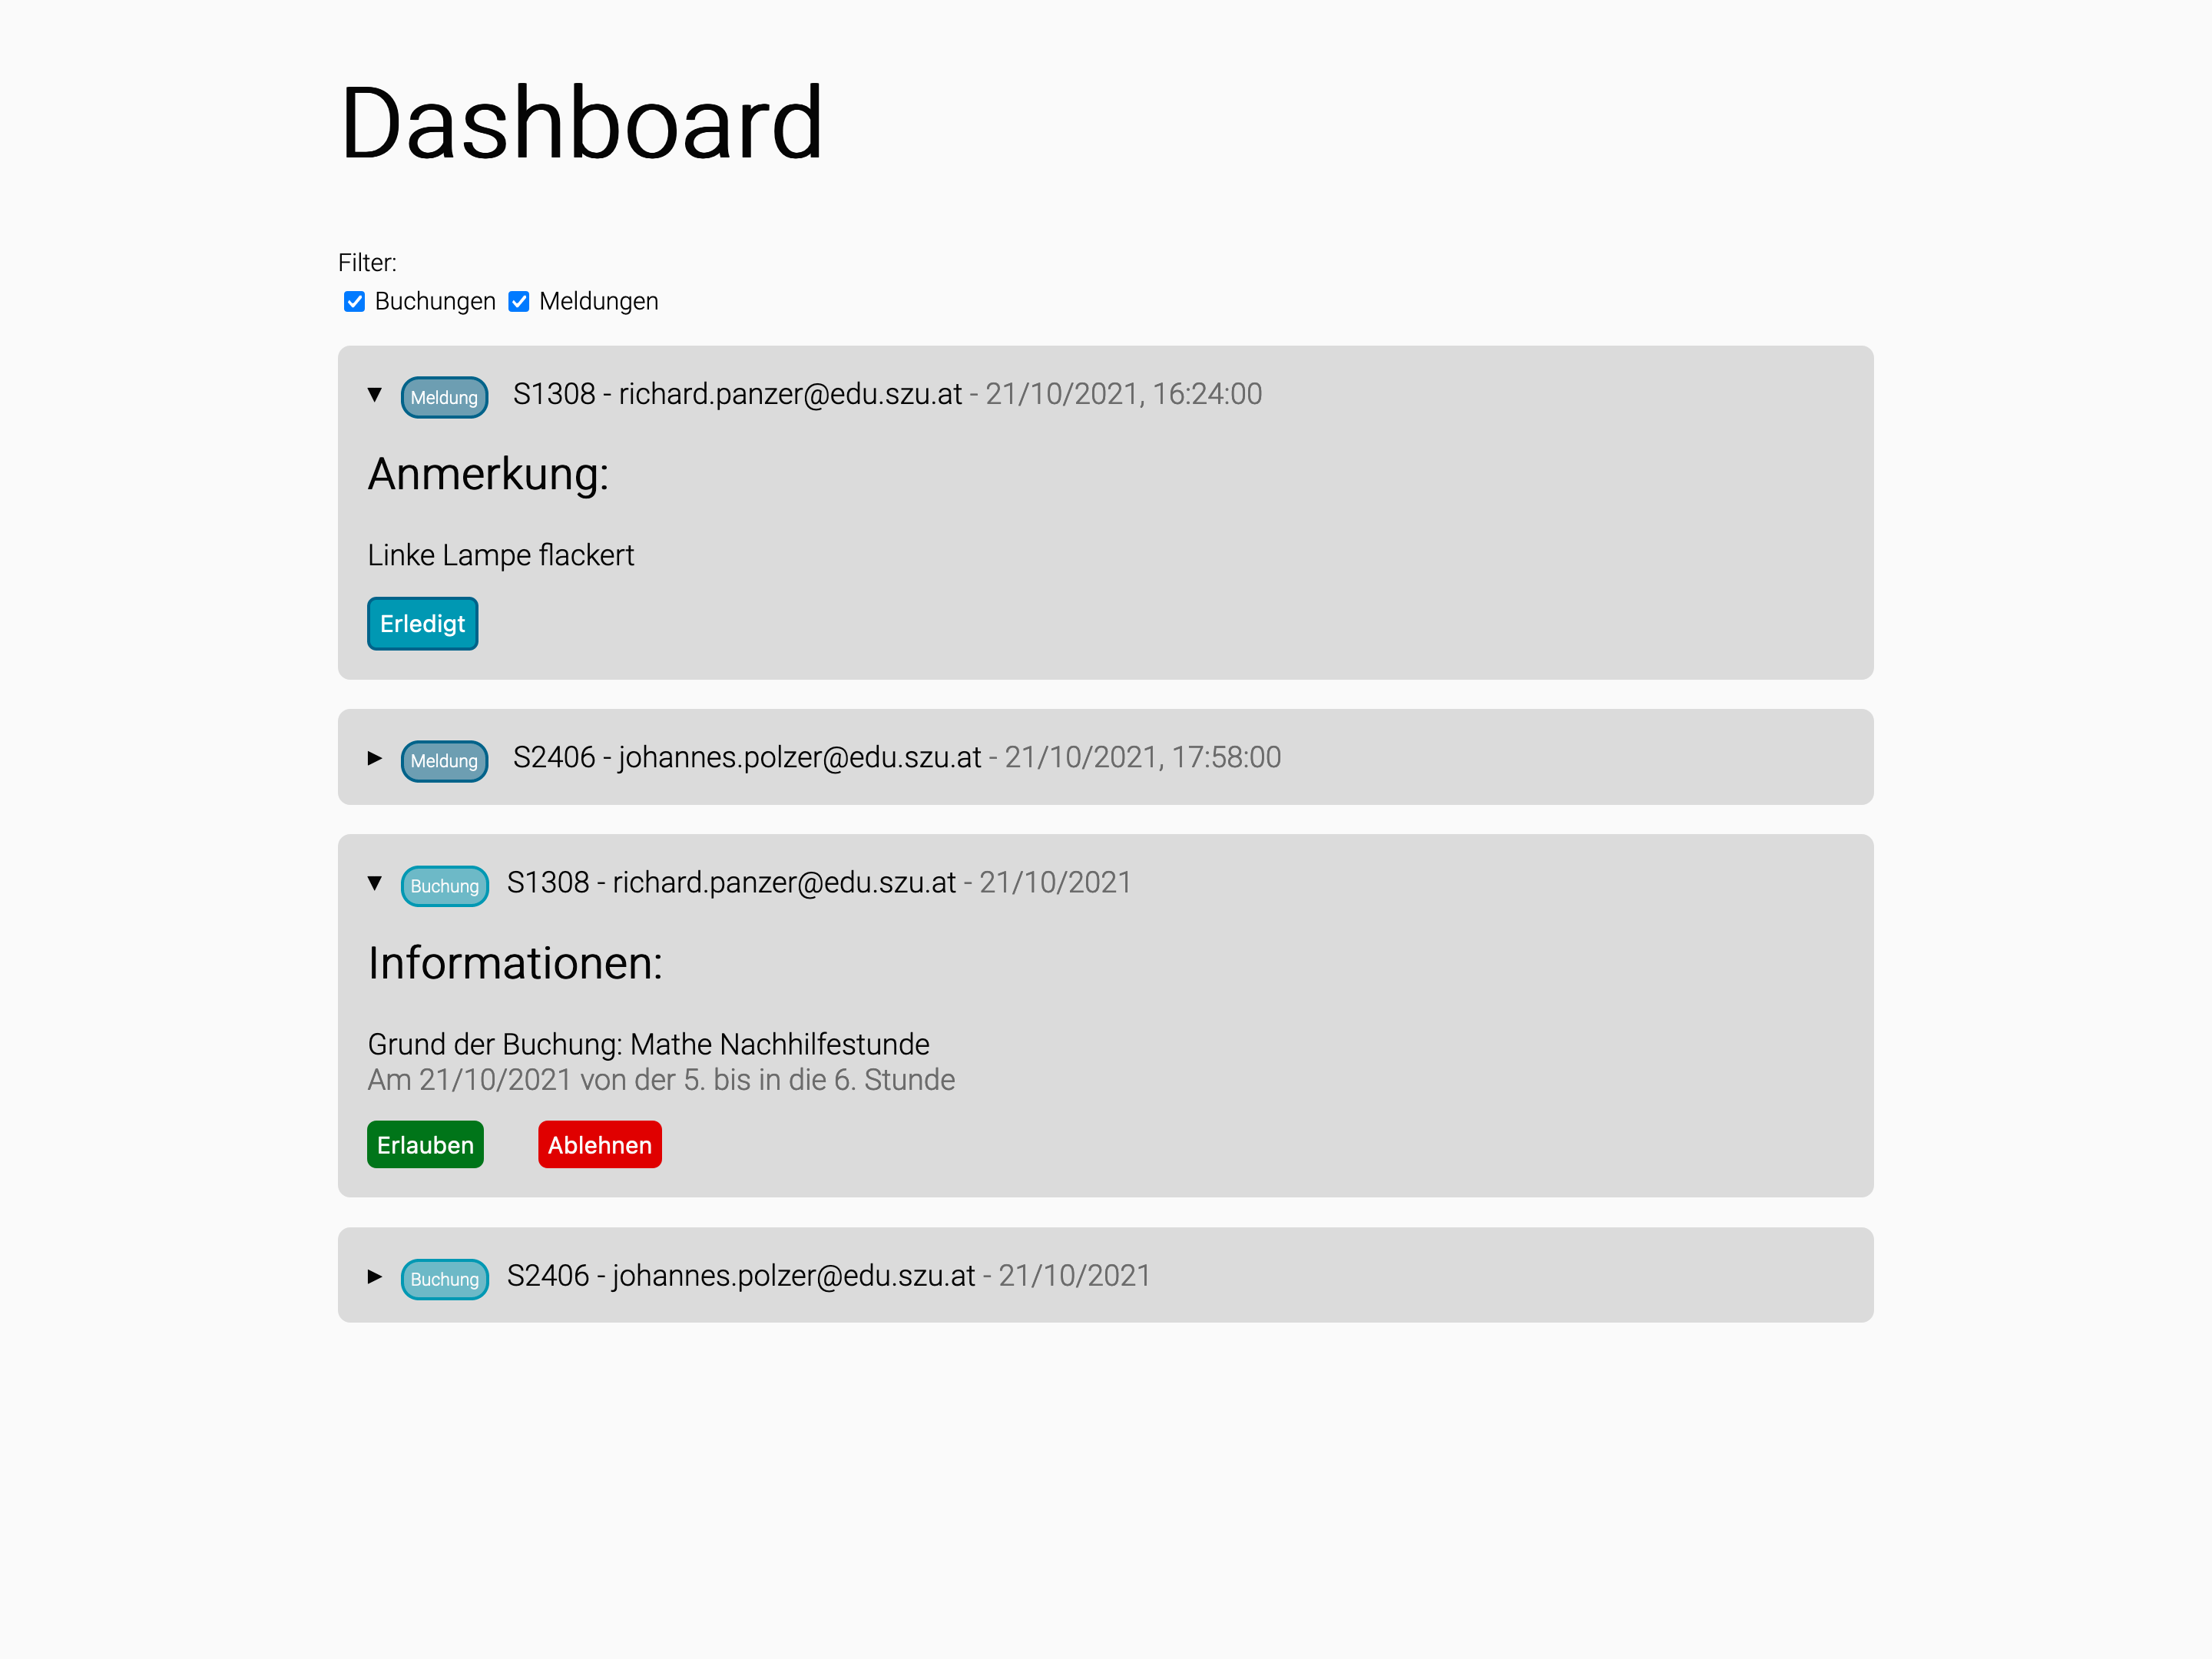
\includegraphics[width=120mm]{media/WebComponents/AdminSeite_light.png}
    \caption{ZELIA Adminübersicht auf Computern}
\end{figure}

Hier können Meldungen abgearbeitet und Buchungsanfrage akzeptiert oder abgelehnt werden.
Für mehr Detail wie das "Admin Dashboard" funktioniert siehe Kapitel "Admin Login" und "Dashboard" \ref{sec:webcomplogdash}.
